\chapter{Latent and Sensible Heat Flux Calculations over First-Year Sea Ice}


%%%    I'M NOT DONE THIS CHAPTER
%%%     PLEASE DONT EDIT THIS CHAPTER YET
%%%    THANK YOU! :) 


\\
\noindent Sarah Y. Murphy$^1$, Von P. Walden$^1$, Hailong Wang$^2$, Stephen R. Hudson$^3$\\

\\
\noindent $^1$Washington State University, Pullman, Washington, USA\\
$^2$Pacific Northwest National Laboratory, Richland, Washington, USA\\
$^3$Norwegian Polar Institute, Fram Centre, Tromsø, Norway\\

\begin{spacing}{1}

\noindent \textbf{Abstract}

 \noindent Sensible and latent heat flux values measured during the N-ICE2015 experiment calculated using LiCor’s EddyPro7 software are used as validation for methods of calculated surface fluxes over first-year sea ice. Fluxes can be calculated using equations based on the Monin-Obukhov similarity theory (bulk flux algorithm) and the more recently developed Maximum Entropy Production method. The Bulk Flux Algorithm is what is typically used in models and is currently used in many atmospheric models. There are parameters present in these equations that represent estimations of surface properties, such as stability, which can be underestimated in the polar regions when strong stability is observed near the surface. Ten different sets of stability-dependent equations for universal functions have been tested for use during the N-ICE field experiment. These universal function values are used in both the bulk flux algorithm and the Maximum Entropy method. The MEP method estimates the surface fluxes without requiring transfer coefficients and empirically defined values. This approach does not require as many measured variables as the bulk approach of calculating these fluxes, resulting in not only an increased ease of use, but also reduces error sources. Both equations have been tested with ten popular sets of equations for the surface stability functions. 
\end{spacing}

\doublespacing
\section{Introduction}

% why is SEB important
Understanding the energy budget at the sea ice surface is of particular importance as small changes in radiation can set off feedback loops that can result in significant climate implications. Reductions in sea ice have been found to amplify the impacts of global warming \cite{wunderling:2020} \cite{ipcc_techsum}. Differences in the surface features and atmospheric conditions present challenges for modeling the surface energy and water balances \cite{wang:2009}. 

\begin{equation}\label{eq:seb}
F_{s} - C = Q_{net} + H_{s} + H_{l}
\end{equation}

% what is the sensible and latent heat flux physically?
The energy budget can be seen in \ref{eq:seb}. The net radiative flux, $Q_{net}$, is the solar and terrestrial radiation, $F_{s}$ is the energy storage, and $C$ is the heat flux from the underlying ocean \cite{walden:2017}. The turbulent fluxes, $H_{s}$ and $H_{l}$, are the sensible and latent heat flux, and are the focus of this paper. Physically, the sensible heat flux represents a chance in temperature. A positive sensible heat flux represents surface warming, as the atmospheric temperatures are warmer than the ice surface. This is often the case during the winter, when advection brings warm air over the frozen surface. Negative sensible heat flux values represent the opposite, the surface is warmer than the atmosphere and is heating the overlying air. Latent heat flux is the heat associated with a phase change; positive latent heat flux is representative of condensation or freezing at the surface, and a negative indicates melting, evaporation, or sublimation.

% measuring SEB
Some components of the energy budget, such as the shortwave and longwave radiation, can be measured directly with radiometers. The sensible and latent heat flux, however, are more difficult to measure. A common approach to taking these measurements is the Eddy Covariance theory, which has been built into LiCor's EddyPro 7 \cite{epro} software for processing flux measurements. This program takes high-frequency measurements of surface fluxes, conducts calibration and filtering, then calculates the sensible and latent heat fluxes, along with $H_{2}0$, $CH_{4}$, $CO_{2}$ and other trace gasses \cite{epro_man}. However, an eddy covariance system is required to take the appropriate measurements to use the Eddy Covariance theory, and without the appropriate system, it is impossible to process the data using EddyPro. 

% field capaigns measuring the SEB
The Norwegian Young Sea Ice Field Campaign (N-ICE) in 2015 and the Surface Heat Budget of the Arctic Ocean Experiment (SHEBA) in 1998 both deployed eddy covariance systems, radiometers, and meteorological towers over sea ice in the Arctic ocean. SHEBA took place over older, multi-year sea ice, and the data collected has been processed both using Eddy Covariance theory and using other methods not requiring the eddy covariance system. N-ICE took place on young, first-year sea ice. A description of the fluxes observed by the eddy covariance system and radiometers can be found in Walden et al., \cite{walden:2017}, which describes the observed surface energy budget at N-ICE in detail. 


\section{Calculating Sensible and Latent Heat Flux}
Sensible and latent heat fluxes for N-ICE were been calculated using LiCor’s EddyPro7 software \cite{epro}. In this paper, the values estimated by EddyPro are compared to two methods of estimating sensible and latent heat flux: a bulk flux algorithm based in Monin-Obukhov similarity theory \cite{foken:2008} and the Maximum Entropy Production method (MEP) \cite{zhang:2021, wang:2014, wang:2009}. Both methods estimate flux without covariance measurements and instead utilize values more commonly observed at weather stations: temperature, moisture, and pressure.

\subsection{Bulk Flux Algorithms}
Algorithms using bulk variables are most commonly used for estimating fluxes \ref{reeves:2021}. Formulations of sensible and latent heat flux are shown in equations \ref{eq:hs} and \ref{eq:hl}. These equations require measurements of temperature and moisture content at two levels of the atmosphere and wind speed. They also require knowledge of exchange coefficients for the underlying surface.
\begin{equation}\label{eq:hs}
H_{s} = - \rho C_{p} U_{*} t_{*} = \rho C_{p} C_{Hz} U_{z} [T_{s} - T_{z}]
\end{equation}
\begin{equation}\label{eq:hl}
H_{l} = - \rho L_{v} U_{*} q_{*} = \rho L_{v} C_{Ez} U_{z} [Q_{s} - Q_{z}] 
\end{equation}
In these equations, $\rho$ is the density of the air, $C_{p}$ the specific heat of air, $U_{*}$ the friction velocity, $t_{*}$ and $q_{*}$ are the temperature and humidity flux scales, and $C_{hz}$ and $C_{Ez}$ are the heat and moisture exchange bulk transfer coefficients \ref{stull:}. Equations \ref{eq:chz} and \ref{eq:cez} are the generally accepted functions for estimating these coefficients. 
\begin{equation}\label{eq:cez}
C_{Ez} = \frac{\kappa C_{D}^{\frac{1}{2}}}{[ln(\frac{r}{z_{Q}})-\varphi_{H}]}
\end{equation}
\begin{equation}\label{eq:chz}
C_{hz} =  \kappa^{2} \left[ ln \left( \frac{z}{z_{0}} \right) - \varphi_{m} \right] ^{-1} \left[ ln \left( \frac{z}{z_{0}} \right) - \varphi_{h} \right] ^{-1}
\end{equation}

These equations are functions of $\varphi_{m}$ and $\varphi_{h}$, the empirical stability functions, which depend on the surface stability. 

\subsection{Maximum Entropy Production Method} 
The MEP method was developed to accurately estimate surface fluxes while limiting the number of empirically derived values and surface transfer coefficients used. This method is based on the principle of maximum entropy (MaxEnt) and Bayesian probability theory from statistical mechanics \cite{dewar:2004, wang:2014}. Equations \ref{eq:mep:hl}, \ref{eq:mep:hs}, and \ref{eq:mep:rn} are the MEP method formulations for sensible ($H_{s}$), latent ($H_{l}$), and surface thermal ($Q$) energy flux, respectively. Equation \ref{eq:mep:b} is a scaling parameter required by both the sensible and latent heat flux calculations. Calculations of sensible and latent heat flux using this method require estimations of the thermal conductivity \cite{wang:2014}. This model has been used to calculate fluxes during SHEBA and was shown to calculate fluxes with some degree of accuracy, proving it's ability to perform in the polar regions \cite{wang:2014}.

\begin{equation}\label{eq:mep:rn}
\left[ 1 + B(\theta) + \frac{B(\theta)}{\theta} \frac{I_{wsi}}{I_{0}} | H_{s} | ^{-\frac{1}{6}} \right] H_{s} = R_{n}
\end{equation}
\begin{equation}\label{eq:mep:hl}
H_{l} = B(\theta) H_{s}
\end{equation}
\begin{equation}\label{eq:mep:hs}
Q = R_{l}^{n} - E - H_{s}
\end{equation}
\begin{equation}\label{eq:mep:b}
B(\theta) = 6 \left( \sqrt{1 + \frac{11}{36}} - 1 \right)
\end{equation}
\begin{equation}\label{eq:iwsi}
I_{wsi} = \sqrt{\rho c \lambda}
\end{equation}
\begin{equation}\label{eq:i0}
I_{0} = \rho c_{p} \sqrt{C_{1}\kappa z} \left( C_{2} \frac{\kappa zg}{\rho c_{p} T_{r}} \right)^{\frac{1}{6}}
\end{equation}

Wang and Bras \cite{wang:2009} use Businger's relationships \cite{businger:1971} to estimate surface exchange coefficients (Businger et al. \cite{businger:1971} in table \ref{tab:stability}), but little has been published about varying the relationship used for these values. 

Thermal conductivity in the MEP method is used to estimate the thermal inertia parameter ($I_{wsi}$ \ref{eq:iwsi}). This equation requires $\rho$ (density), $c$ (specific heat), and $\lambda$ (thermal conductivity). Merkouriadi et al. \cite{merkouriadi:2017} found that the thermal conductivity of snow on sea ice during N-ICE2015 was much lower than those used in many modeling studies. Chapter 4 takes a deeper look the importance of having an accurate estimate of these values over first-year sea ice. 

\subsection{Surface Stability}

Some commonly accepted sets of equations for the empirical stability coefficients are shown in table \ref{tab:stability}. These equations use the Obukhov number (equation \ref{eq:zl}) to determine surface stability. Positive Obukhov numbers indicate stable conditions and negative indicate unstable conditions. Some relations find that using a von-Kármán constant ($\kappa$) of $0.35$ can improve calculations, but changing this variable is outside the scope of this study, so only formulations using $\kappa = 0.4$ to calculate $\zeta$ are included in table \ref{tab:stability}. 

Each of the equations shown in the table have different ranges of stability for which they can be applied. These are formulated empirically, meaning they depend on measurements and are useful only under similar conditions \cite{stull:} \cite{foken:2008}. Many of these equations, with the exception of Andreas et al. \cite{andreas:2010} were created under conditions observed in mid-latitudes. Andreas et al. \cite{andreas:2010}, on the other hand, used results from the SHEBA field experiment to tune the relationships based on the Businger-Dyer-Pandolpho (BDP) relationship (equation \ref{eq:bdp:m} and \ref{eq:bdp:H}. This relationship is generally used for neutral and unstable conditions \cite{foken:2008}, so it requires tuning for other locations. Unlike many of the equations in table \ref{tab:stability}, the BDP relationship requires an extra variable, $\gamma$, which is defined empirically for each location.

\begin{equation}\label{eq:bdp:m}
\varphi_{m}(\zeta) = (1 + \gamma \zeta)^{-1/4}
\end{equation}

\begin{equation}\label{eq:bdp:H}
\varphi_{H} = \begin{cases} 
\varphi_{m} & \text{    } \zeta \geq 0 \\ 
\varphi_{m}^{2} & \text{    } \zeta < 0 \\ 
\end{cases}
\end{equation}

The polar regions experience stronger surface inversions than in lower-latitude locations, and sometimes the stability seen in these locations is too low for other empirical stability functions to apply, or, if they do claim to be valid under those conditions, they may have little validation for Obukhov numbers that high. Under these strongly stable conditions, some methods of estimating the scaling parameters break down. 

\begin{equation}\label{eq:zl}
\zeta = \frac{z}{L}
\end{equation}
\begin{equation}\label{eq:l}
L = \frac{u_{*}^{3}}{\kappa \frac{g}{T} \frac{Q_{H}}{\rho C_{p}}}
\end{equation}

% this table is super large but I'm not positive what the best way to fix it would be. Maybe I need to split it into two tables? 

{\rowcolors{2}{gray!25}{}
\begin{table}[p]
\center
\centering
\vspace{-6em}
\small
    \begin{tabular}{| c | c |}
    \hline
        \textbf{Author} & \textbf{Equations} \\ \hline
        Swainbank (1986) \cite{foken:2008} & \shortstack{$\varphi_{m} = \begin{cases} 0.613(-\zeta)^{-0.2} & \text{    } -0.1 \geq \zeta \geq -2 \\ \end{cases}$ \\ $\varphi_{H} = \begin{cases} 0.226 (-1/L)^{-0.44} & \text{    } -0.1 \geq \zeta \geq -2 \\ \end{cases}$} \\ 
        
        Tschalikov (1968) \cite{foken:2008}  & \shortstack{$\varphi_{m} = \begin{cases} 1 + 7.74\zeta & \text{    } \zeta \geq 0.04 \\ \end{cases}$\\$\varphi_{H} = \begin{cases} 1 + 5.17\zeta & \text{    } \zeta \geq 0.04 \\ \end{cases}$ } \\ 
        \shortstack{Zilitinkevich and \\ Tschalikov (1968) \cite{zilitinkevich:1968}}  & \shortstack{$\varphi_{m} = \begin{cases} 1 + 1.38 \zeta & \text{    } -0.15 < \zeta < 0 \\ 0.42(-\zeta)^{1/3} & \text{    } -1.2 < \zeta < -0.15 \\ 1 + 9.4 \zeta & \text{    } 0 < \zeta \\ \end{cases}$\\$\varphi_{H} = \begin{cases} 1 + 1.31 \zeta & \text{    } -0.15 < \zeta < 0 \\ 0.41(-\zeta)^{-1/3} & \text{    } -1.2 < \zeta < -0.15 \\ 0.95 + 8.9 \zeta & \text{    } 0 < \zeta \\ \end{cases}$ } \\ 
        Businger et al. \cite{businger:1971}  & \shortstack{$\varphi_{m} \begin{cases} (1 - 19.3 \zeta)^{-1/4} & \text{    } -2 < \zeta < 0 \\ 1 + 6\zeta & \text{    } 0 < \zeta < 1 \\ \end{cases}$\\$\varphi_{H} \begin{cases} 0.95(1 - 11.6 \zeta)^{-1/2} & \text{    } -2 < \zeta < 0 \\ 0.95 + 7.8\zeta & \text{    } 0 < \zeta < 1 \\ \end{cases}$ } \\ 
        Dyer (1974) \cite{dyer:1974} & \shortstack{$\varphi_{m} \begin{cases} (1 - 15.2 \zeta)^{-1/2} & \text{    } -1 < \zeta < 0 \\ 1 + 4.8\zeta & \text{    } 0 < \zeta \\  \end{cases}$ } \\ 
        Skeib (1980) \cite{foken:1990} & \shortstack{$\varphi_{m} = \begin{cases} 1 & \text{    } -0.0625 < \zeta < 0.125 \\ (\frac{\zeta}{-0.0625})^{-1/4} & \text{    } -2 < \zeta < -0.0625 \\ \frac{\zeta}{0.125} & \text{    } 0.125 < \zeta < 2 \\ \end{cases}$\\$\varphi_{H} = \begin{cases} 1 & \text{    } -0.0625 < \zeta < 0.125 \\ 0.95(\frac{\zeta}{-0.0625})^{-1/2} & \text{    } -2 < \zeta < -0.0625 \\ 0.95(\frac{\zeta}{0.125})^{2} & \text{    } 0.125 < \zeta < 2 \\ \end{cases}$ } \\ 
        \shortstack{Gavrilov and \\ Petrov (1981) \cite{gavrilov:1981}}  & \shortstack{$\varphi_{m} = \begin{cases} (1-8\zeta)^{-1/3} & \text{    } \zeta < 0\\ 1 + 5 \zeta & \text{    } 0 < \zeta\\ \end{cases}$\\$\varphi_{H} = \begin{cases} 0.65 \left[ (1-35\zeta)^{-1/2} + \frac{0.25}{1+8(\zeta)^{2}} \right] & \text{    } \zeta < 0\\ 0.9 + 6 \zeta & \text{    } 0 < \zeta\\ \end{cases}$ } \\ 
        \shortstack{Dyer and \\ Bradley (1982) \cite{dyer:1982}}  & \shortstack{$\varphi_{m} = \begin{cases} (1 - 28\zeta)^{-1/4} & \text{    } \zeta < 0 \\ \end{cases}$\\$\varphi_{H} = \begin{cases} (1 - 14\zeta)^{-1/2} & \text{    } \zeta < 0 \\ \end{cases}$ } \\ 
        \shortstack{Beljaars and \\ Holtslag (1991) \cite{beljaars:1991}}  &\shortstack{$\varphi_{m} = \begin{cases} 1 + \zeta + \frac{2}{3} \zeta (6 - 0.35 \zeta) e^{-0.35} \zeta & \text{    } \zeta < 0 \\ \end{cases}$\\$\varphi_{H} = \begin{cases} 1 + \zeta + (1_+ \frac{2}{3} \zeta)^{1/2} (6 - 0.35 \zeta) e^{-0.35 \zeta} & \text{    } \zeta < 0 \\ \end{cases}$ } \\ 
        Handorf et al. (1999) \cite{handorf:1999} & \shortstack{$\varphi_{m} = \begin{cases} 1 + 5 \zeta & \text{    } 0 < \zeta < 0.6 \\ 4 & \text{    } \zeta > 0.6 \\ \end{cases}$\\$\varphi_{H} = \begin{cases} 1 + 5 \zeta & \text{    } 0 < \zeta < 0.6 \\ 4 & \text{    } \zeta > 0.6 \\ \end{cases}$ } \\ 
        Andreas et al. \cite{andreas:2009} & \shortstack{$\varphi_{m} = \begin{cases} BDP(\gamma = 16) & \text{    } z/L < 0 \\ -5z/L & \text{    } z/L \geq 0 \\ \end{cases}$ \\ $\varphi_{H} = \begin{cases} \varphi_{m}^{2} & \text{    } z/L < 0 \\ \varphi_{m} & \text{    } z/L \geq 0 \\ \end{cases}$ } \\ 
        \hline
    \end{tabular}
    \caption{Stability Equations from Micrometeorology \cite{foken:2008} for the universal functions of momentum and heat. $L$ is the Obukhov-Length and $z$ the measurements height. BDP represents the Businger-Dyer-Pandolfo relationship\cite{foken:2008}.}
    \label{tab:stability}
\end{table}}

\section{Methods}
Atmospheric measurements of temperature, wind speed, and atmospheric humidity at N-ICE were taken continuously at three levels ($2 m$, $4 m$, and $10 m$) from a meteorological tower constructed on the sea ice. Pressure was reported at sea level, and for this study was used to calculate the $2 m$, $4 m$, and $10 m$ pressure using the barometric equation \cite{lente:2020}. Moisture was measured and reported as relative humidity and was converted to saturation vapor pressure and specific humidity using the Clausius-Clapeyron equation \cite{iribarne:2981}, surface temperature, and relative humidity. The bulk algorithm requires two levels of specific humidity, but the MEP formulation only requires the surface variables, making it easier to use on experiments with only one measurement level, so the surface specific humidity was calculated for this. All height levels of relative humidity were converted to specific humidity so each measurement level could be used in the bulk algorithm for comparison. 

\section{Results and Discussion}

\subsection{Stability Coefficients}
To determine the stability, equation \ref{eq:zl} was calculated from observations at N-ICE. While we do have covariance measurements for the entire time period, this study avoids using those in these values to showcase the ability to calculate fluxes in situations where these are not available. Figure \ref{fig:ol} shows the Obukhov length ($L$, \ref{eq:l}) during N-ICE and that calculated by EddyPro. This preliminary comparison was done to determine if any sources of error could be attributed to errors in the Obukhov length. The EddyPro estimation of Obukhov length produced slightly more negative (unstable) values than those calculated by equation \ref{eq:l}. 

\begin{figure}[H]
    \centering
    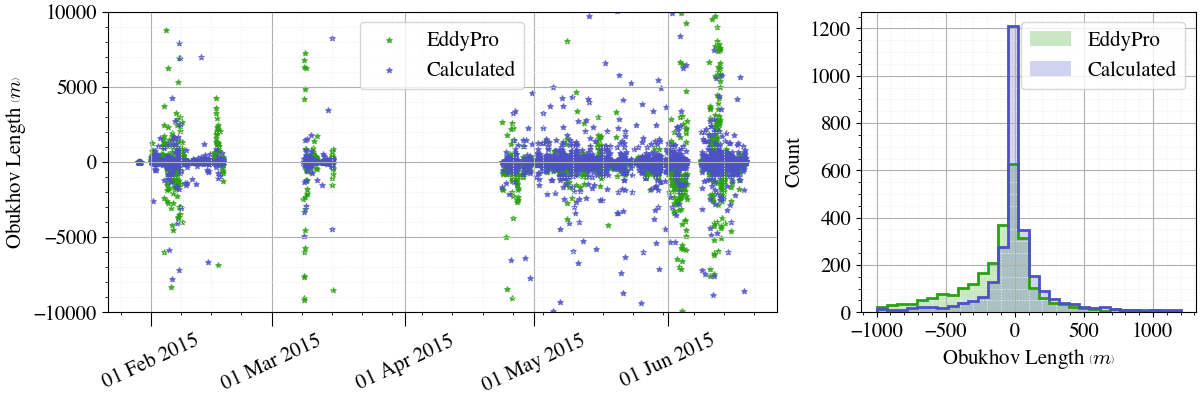
\includegraphics[width=1\linewidth]{figures/chapter3/ch3_obukhovlength.png}
    \caption[Obukhov length]{The Obukhov length measured during N-ICE and processed using EddyPro (EddyPro, blue) and calculated using equation \ref{eq:l} (Calculated, maroon).}
    \label{fig:ol}
\end{figure}

Obukhov length depends on the friction velocity, and the surface below N-ICE is first-year sea ice, a flat surface with limited sources of mechanical turbulence. The mean roughness length observed at N-ICE was $0.005 m$ with a standard deviation of $0.0216 m$. Roughness length can be entered into the EddyPro system and a constant value of xxx was used. 


\begin{table}[H]
\centering
{\rowcolors{4}{}{gray!25}
\begin{tabular}{| c | c | c | c | c | c |}
 \hline
\multirow{3}{*}{\textbf{Author}} & \multicolumn{4}{c|}{\textbf{Mean Error $\left(W m^{-2}\right)$}} &  \multirow{3}{*}{\textbf{N}} \\
  & \multicolumn{2}{c|}{\textbf{MEP}} & \multicolumn{2}{c|}{\textbf{Bulk}} & \\
  & $H_{l}$ & $H_{s}$ & $H_{l}$ & $H_{s}$ & \\
 \hline
 Swainbank & 3.0702 & 158.9661 & 0.5229 & 9.8116 & 99 \\ 
 Tschalikov & 7.5555 & 49.6636 & -65.1821 & 104.1411 & 247 \\  
 Zilitinkevich and Tschalikov & 3.2457 & 175.9534 & -36.7010 & -70.3093 & 1547 \\
 Businger et al. & 2.7981 & 178.4340 & -38.4473 & 304.4379 & 1523 \\
 Dyer & 2.3268 & 192.7868 & -31.2514 & -9.6833 & 1368 \\
 Skeib & 2.4796 & 177.0861 & -38.6380 & -8.3428 & 1406 \\
 Gavrilov and Petrov & -2.3067 & 114.6652 & -37.1897 & 120.2434 & 559 \\
 Dyer and Bradley & 6.2988 & 207.9137 & -35.5161 & -14.9588 & 1006 \\
 Beljaars and Holtslag & -2.6742 & 114.6421 & -36.9582 & 45.4032 & 559 \\
 Handorf et al. & -2.5078 & 114.6465 & -36.9910 & 39.0398 & 559 \\
 Andreas et al. & -0.8821 & 175.1623 & -36.2989 & -5.0711 & 1565 \\
 \hline
\end{tabular}}
\caption{Mean error sensible and latent heat flux calculations using each stability equation listed in table \ref{tab:stability} for both the MEP equations and the Bulk Flux algorithm. The number of hourly measurements in the applicable ranges is shown in the rightmost column.}
\label{tab:stability_error}
\end{table}

Table \ref{tab:stability_error} shows the mean error when using the MEP and Bulk Flux methods to calculate surface fluxes when compared to the EddyPro results. Each source in the "Author" column corresponds to equations in table \ref{tab:stability}. Each has a different number of hourly measurements included because each is applicable to specific ranges in stability. For example. Swainbank \cite{foken:2008} is only valid for Obukhov numbers between -0.1 and -2, indicating this is only valid for stable conditions, which we see rarely in the polar regions, resulting in a small number of observations used. Andreas et al. \cite{andreas:311}, on the other hand, was created using the SHEBA observations and has the largest range of value it is valid over. The equations created by Andreas et al. \cite{andreas:311} had the lowest mean error for the latent heat flux when using the MEP equation, however it's performance calculating the sensible heat flux was comparable to other equations considering the same wide range of stability values. 

Using the Bulk Flux algorithm resulted in fairly similar values of error for latent heat flux regardless of universal function relationships used with the exception of the Swainbank and Tschalikov \cite{foken:2008} formulations, which had a significantly lower and higher mean error, respectively. While Swainbank \cite{foken:2008} did have the lowest mean error for the latent heat flux and one of the lowest for the sensible heat flux, it was not selected for use because of the low number of stability conditions it can be used over.  

Due to it's wide range of stability values and it's improved performance for latent heat flux, the Andreas et al. \cite{andreas:2010}, formulation was used for the final analysis of both the Bulk Flux equation and the MEP equation. The MEP equation typically uses the relations developed by Businger et al. \cite{businger:1971}, but for our location the Andreas \cite{andreas:311} formulation performed better when compared to the EddyPro measurements when calculating latent heat flux. Sensible heat flux, on the other hand, was comparable between the Andreas \cite{andreas:311} formulation and the Businger et al. \cite{businger:1971} formulation. 


\subsection{Thermal Conductivity}
Thermal conductivity is used in the MEP method to calculate the thermal inertia parameter, as shown in equation \ref{eq:iwsi}. Thermal conductivity values at N-ICE were much lower than those commonly used in models \cite{merkouriadi:2017}, so special care was taken to ensure the thermal conductivity estimate was accurate for our conditions. Using the thermal conductivity values shown in table \ref{tab:thermal} with equation \ref{eq:iwsi}, we estimate the thermal inertia parameter at N-ICE as shown in table \ref{tab:thermal}. 

\begin{table}[H]
\centering
{\rowcolors{2}{gray!25}{}
\begin{tabular}{| c | c | c |}
 \hline
\multirow{2}{*}{\textbf{Floe}} & \textbf{Thermal Inertia} & \textbf{Thermal Conductivity} \\
  & $(m^{-1} \space K^{-1})$ & $(J m^{-2}Ks^{-1/2})$ \\
  \hline
 1 & 0.1830 & 314.2636  \\
 2 & 0.2457 & 429.6496 \\ 
 3 & 0.1915 & 280.4235 \\
 4 & 0.3105 & 1009.8157 \\
  \hline
\end{tabular}}
\caption{Thermal inertia for each floe during N-ICE. Conductivity values were taken as a mean from \cite{merkouriadi:2017} (winter) and Gallet et al. \cite{gallet:2017} (spring) and inertia parameters were calculated using equation}
\label{tab:thermal}
\end{table}

 \subsection{Maximum Entropy Method}

\begin{figure}[H]
    \centering
    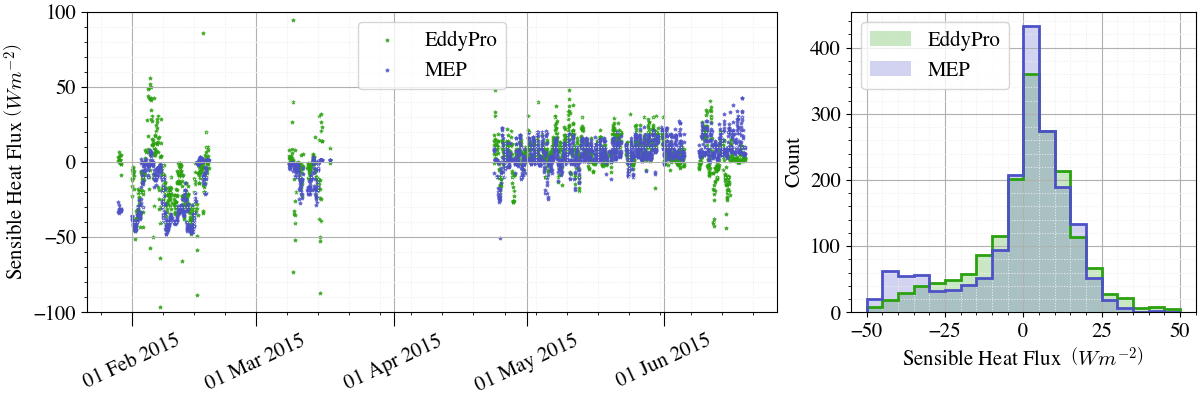
\includegraphics[width=1\linewidth]{figures/chapter3/MEPSensible.png}
    \caption[Sensible heat flux from the MEP method compared to EddyPro]{The sensible heat flux at N-ICE as calculated with EddyPro (green) and with the MEP method (blue).}
    \label{fig:mep:sensible}
\end{figure}

\begin{figure}[H]
    \centering
    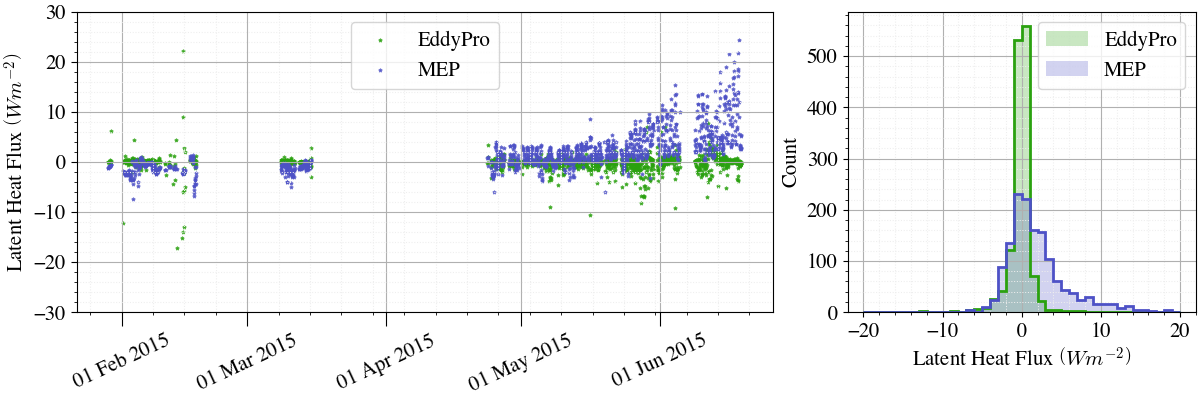
\includegraphics[width=1\linewidth]{figures/chapter3/MEPLatent.png}
    \caption[Latent heat flux from the MEP method compared to EddyPro]{The latent heat flux at N-ICE as calculated with EddyPro (green) and with the MEP method (blue).}
    \label{fig:mep:latent}
\end{figure}

Sensible heat flux from the MEP method is obtained using equation \ref{eq:mep:hs}. The results of this are shown in figure \ref{fig:mep:sensible}. The results using this method accurately represented the sensible heat fluxes at N-ICE for most of the experiment. In the winter, fluxes were slightly underestimated by the MEP equation, resulting in a bi-modal shape to the distribution shown on the right of the figure. In the spring, there was one occurrence lasting several days with largely negative sensible heat flux shown in the EddyPro results wile the sensible heat fluxes from the MEP equation stayed positive. 

Latent heat fluxes (figure \ref{fig:mep:latent}) were not represented as closely in the MEP to the EddyPro output. EddyPro showed very small latent heat fluxes throughout the entire experiment. These small heat fluxes were surprising and are not captured with the MEP method. February and March values of latent heat flux are comparable between the MEP and EddyPro calculations, but during spring and entering summer MEP values are at times $20 Wm^{-2}$ greater than those calculated by EddyPro, which are rarely greater than $10 Wm^{-2}$.

 \subsection{Bulk Flux Algorithm}
\begin{figure}[H]
    \centering
    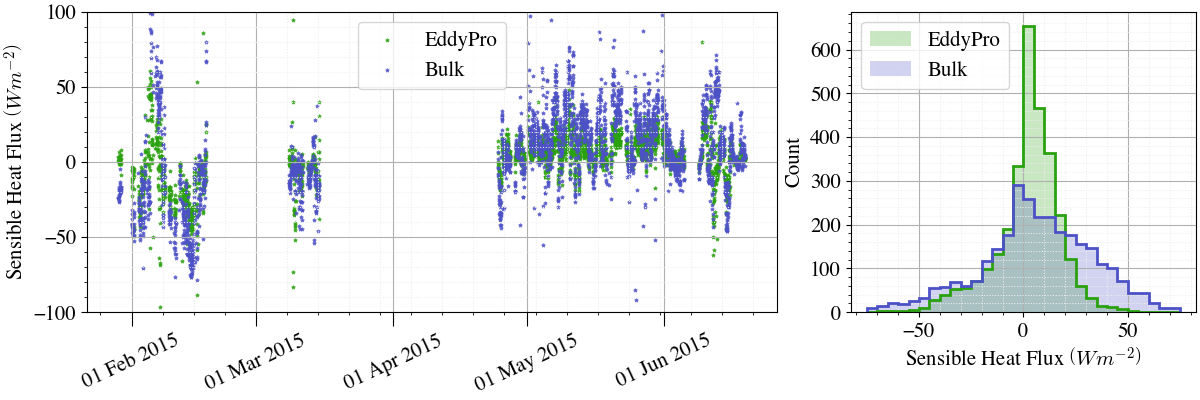
\includegraphics[width=1\linewidth]{figures/chapter3/BulkSensible.png}
    \caption[Sensible heat flux from a bulk flux method compared to EddyPro]{The sensible heat flux at N-ICE as calculated with EddyPro (green) and with a bulk flux algorithm method (blue).}
    \label{fig:bulk:sensible}
\end{figure}
\begin{figure}[H]
    \centering
    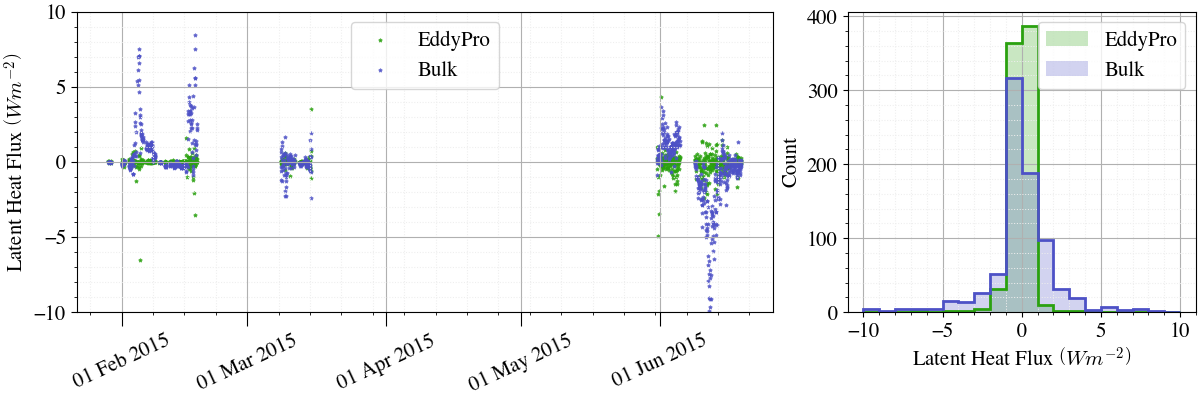
\includegraphics[width=1\linewidth]{figures/chapter3/BulkLatent.png}
    \caption[Latent heat flux from a bulk flux method compared to EddyPro]{The latent heat flux at N-ICE as calculated with EddyPro (green) and with a bulk flux algorithm method (blue).}
    \label{fig:bulk:latent}
\end{figure}

Calculating the fluxes using the bulk flux algorithm resulted in more largely positive values than was represented in the EddyPro results and in the MEP results. These can be seen in figure \ref{fig:bulk:sensible}. In spring the sensible heat flux is consistently over estimated by the Bulk algorithm, indicating the temperature difference between the surface and the atmosphere is too large in the calculations, and too much head is being transferred in to the surface. The latent heat flux, shown in figure \ref{fig:bulk:latent}, was also calculated to be significantly larger than the EddyPro results when using the bulk flux algorithm. 

In June, there was a large decrease in the latent heat flux according to the bulk algorithm. This was mirrored by an increase in the sensible heat flux. However, this decrease (increase) in the latent heat flux (sensible heat flux) was not shown in the EddyPro method. EddyPro produced latent heat flux values consistently around zero during this time period, while the sensible heat flux dropped. This indicates that the air was cooler than the surface and sensible heat transfer occurred instead of a phase change. However, the bulk flux algorithm favored a phase change, likely melting, over a sensible heat flux change. At this time in the experiment, there likely was significant phase change occuring as many melt ponds were developing in the surrounding area \cite{walden:2017}. Overall, latent heat flux values estimated by the Bulk equation are more largely positive in the winter and more largely negative in the summer, indicating the Bulk flux algorithm shows more melting in the spring and more freezing in the winter than the EddyPro results. 

Positive latent heat flux values in the winter represent surface freezing. These values are, at times, almost $10 Wm^{-2}$ greater in the Bulk results than in the EddyPro results. EddyPro, once again, favors sensible heat flux changes to phase change. However, the sensible heat flux in the bulk algorithm and in EddyPro are comparable. This indicates that EddyPro is not just favoring the heat transfer to be in the form of sensible heat flux, but it also underestimates the latent heat flux in general, even in situations when it cannot be described by an offset in the sensible heat flux. 

%% SENSIBLE
% positive - surface warming (air warmer than sfc) if sfc correct air too warm
% negataive - surface cooling (air cooler than sfc) if sfc correct air too cold

%% LATENT
% positive - freezing
% negative - melting

\section{Summary and Conclusions}
Sensible and latent heat flux formulations require high temporal resolution to use eddy covariance methods. Two methods of calculating sensible and latent heat flux that do not require and eddy covariance measurements are explored here. The MEP method, a method utilizing the thermal conductivity, net radiative flux, and  the stability. The bulk flux method requires measurements of moisture and temperature at two levels, the wind speed, and stability. Both equations require the bulk transfer coefficients of heat and moisture, which are a function of the stability and have been empirically defined for experiments over a variety of surfaces. Very few of these functions are appropriate for the strong stabilities that often occur in the polar regions. Andreas et al., \cite{andreas:311} developed a relationship for these functions that applies to strong stabilities seen at SHEBA over multi-year sea ice. This relationship was found to be appropriate for the bulk transfer coefficients at N-ICE using both the bulk flux method and the MEP method. 

The MEP method performed well when compared to the EddyPro values for both sensible and latent heat fluxes. In the winter, the latent heat flux values calculated by the MEP equation are much higher than those in EddyPro, indicating significant more phase change. The bulk method also represented the EddyPro values fairly well, though the MEP formulations does seem to represent the spread of flux values better than the bulk algorithm. The latent heat flux values were also much larger than those observed during N-ICE in the bulk method. 

Overall, further testing is needed for validation of the latent heat flux formulations. The latent heat flux values measured at N-ICE were much smaller than expected, and smaller than those seen at other experiments, so more measurements are needed to determine if this is something that can be expected. Both sensible heat flux formulations, however, produced reasonable values over the first-year sea ice seen at N-ICE. 